\chapter{Interactive Analysis and Decision Support with MATSim}
\label{ch:businessanalytics}
% ##################################################################################################################

\hfill \textbf{Authors:} Alexander Erath and Pieter Fourie

\begin{center} 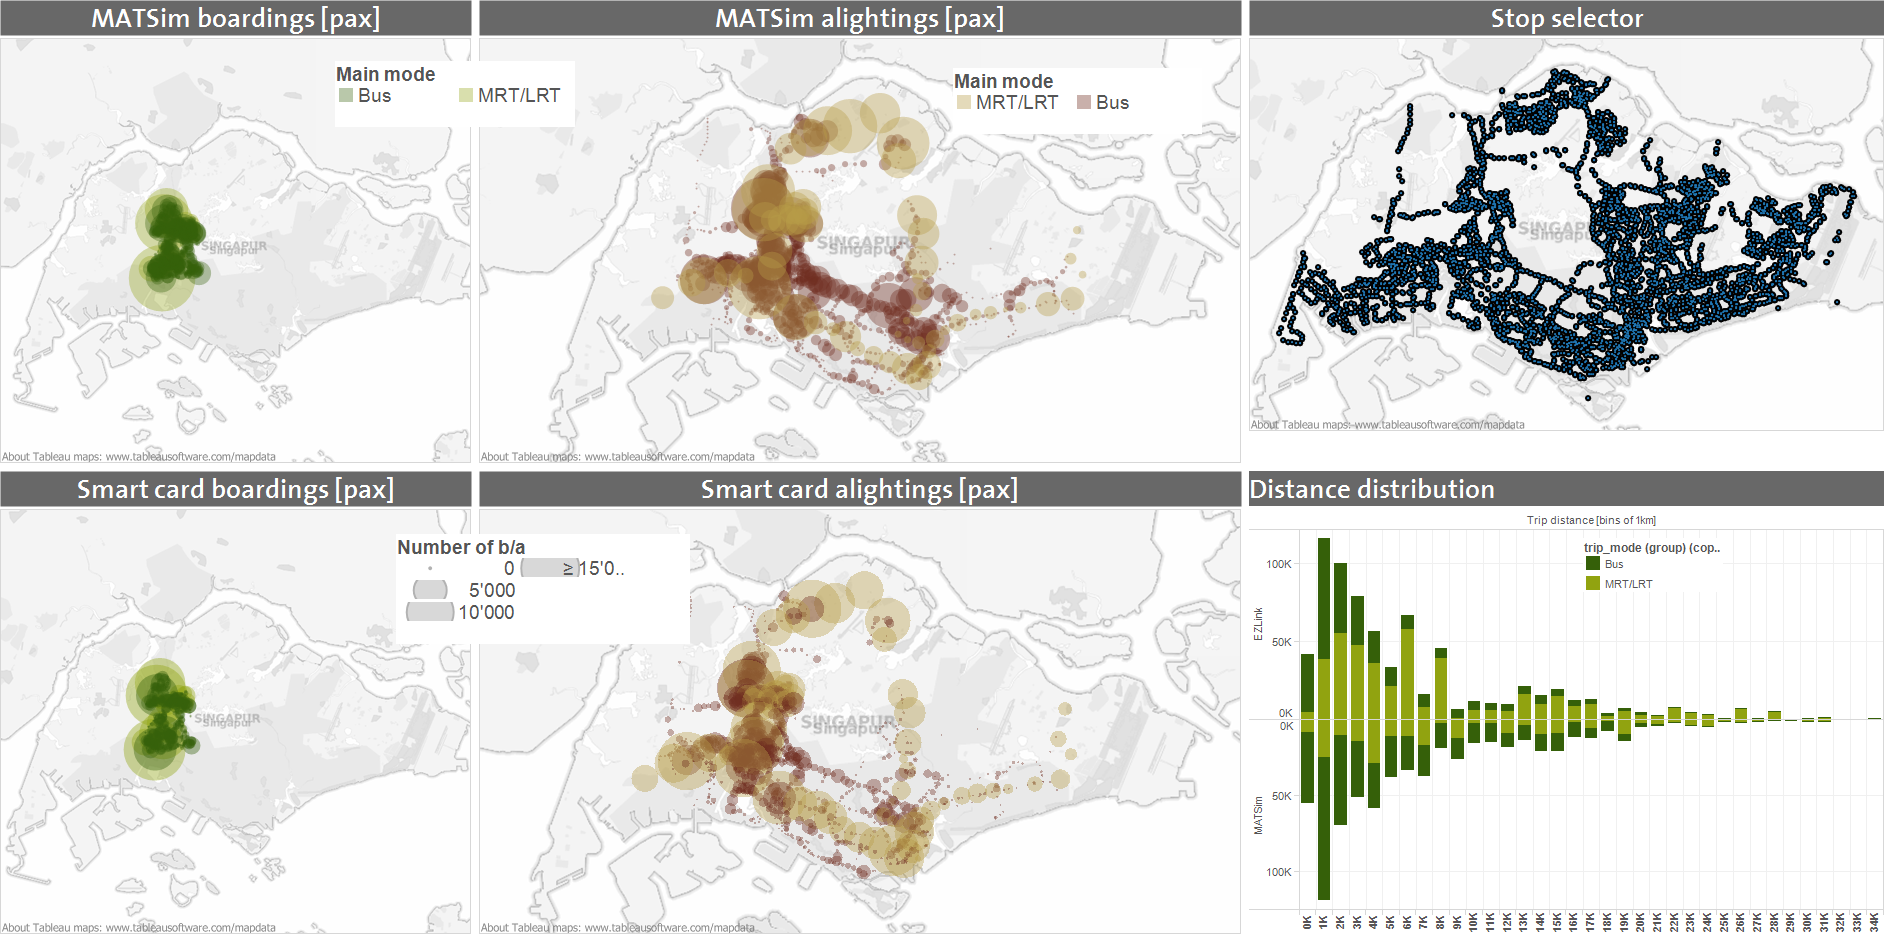
\includegraphics[width=0.4\textwidth, angle=0]{extending/figures/businessanalytics/tableau.png} \end{center}

This chapter is largely based on work in \citet[][]{ErathEtAl_EASTS_2013} where the interested reader will find references to further reading.
\section{Introduction}
\label{sec:analyticsIntro}
\paragraph{Agent-based simulation means lots of data}
Agent-based transport demand models require managing and integrating data sources that are several orders of magnitude larger than traditional aggregate models. In a truly disaggregate demand description, as can be found in our implementation of MATSim for Singapore, spatial data is at the level of individual buildings and land parcels, not zones; and travel demand takes the form of a full activity diary with connecting trips for every individual, based on their personal demographic attributes, instead of an aggregate number of trips from zone to zone for a time period under study. For this reason, the input data for an aggregate four-step (or related) demand model can generally be edited on a laptop using standard spreadsheet software, whereas agent-based modeling requires the manipulation and synthesis of large stores of structured, hierarchical data, frequently exceeding the capacity of most personal computers.

\paragraph{How MATSim stores data}
MATSim stores and retrieves data from XML, because XML can reflect the hierarchical structure of objects in the simulation, and is human-readable. But performing general exploratory analysis of large stores of XML data is usually poorly supported by most data analysis software packages, especially GIS-based systems. In order to perform analyses, expert knowledge of XML querying technologies like XPath and XQuery is required (or Java if one is to perform more specialized analysis on the objects themselves).  It is our experience that this specialized knowledge is lacking in transport and urban spatial planning practice. Therefore, in most applications of MATSim so far, authorities and other interested parties have to formulate their desired analysis in advance and have expert consultancies perform the analysis. Any queries resulting from the analysis means another cycle of consultation, and the value proposition to the client shrinks due to a lack of interactivity and feeling of ownership of the model. From our experience, this lack of a widely supported exploratory data analysis interface and the customer experience it creates, presents a considerable barrier to entry for many authorities and operators that are otherwise interested in using MATSim.

\paragraph{How customers interact with data: relational databases, GUI-driven interaction}
Most customers in the field of transport and urban spatial planning rely on mature, GUI-driven software such as ArcGIS \citep{ARC_GIS_2011}, EMME/3 \citep{EMME_Webpage_2015}, the PTV \citep{PTV_Webpage_2009} transport planning suite, even Microsoft Excel; all of which are capable of connecting to relational databases to perform queries on large datasets. Many analysts are capable of querying databases explicitly using the Structured Query Language (SQL), and the Open Database Connectivity (ODBC) standard allows software to connect to any relational database while being agnostic of the actual technology driving it. Importantly, many interactive exploratory data analysis software suites such as Tableau, Tibco Spotfire,  SAS and the open source R project support relational databases and ODBC.

\section{Requirements of a decision support interface to MATSim}
\label{sec:analyticsRequirements}
The event stream produced by the MATSim mobility simulation is a representation of what happened in the transport simulation at the atomic level. It could be fed into a relational database and an analyst knowledgeable in procedural languages could process it in arbitrary ways. But we foresee that there are general use case scenarios where most analysts will perform general tasks that can be standardized. To this end, we set about compiling a requirements specification of possible audiences and their use case scenarios, to come up with a general framework for interactive analysis and decision support that will satisfy most requirements. We developed a set of Java classes to process MATSim input and output in order to produce the tables in a relational database, according to an entity relationship diagram that should be intuitive and useful to a large user audience.

\subsection{Users}
The decision support tool presented in this chapter is geared to decision makers and researchers
in the fields of transport planning and operations, spatial planning and spatial economics and
geography. Generally speaking, it should serve professionals who are interested in mobility
and spatial analysis and understand the principles of transport modelling but do not have the
expertise to operate an agent-based transport simulation directly. Currently, we envision the
following stakeholders and some example questions for our decision-support system --- a non-exhaustive list that, we expect, will grow with time:


% ------------
\createfigure%
{Tableau visualization}%
{Tableau visualization of public transport ridership from a MATSim simulation compared against actual smart card data records in Singapore}%
{\label{fig:analyticsTableau}}%
{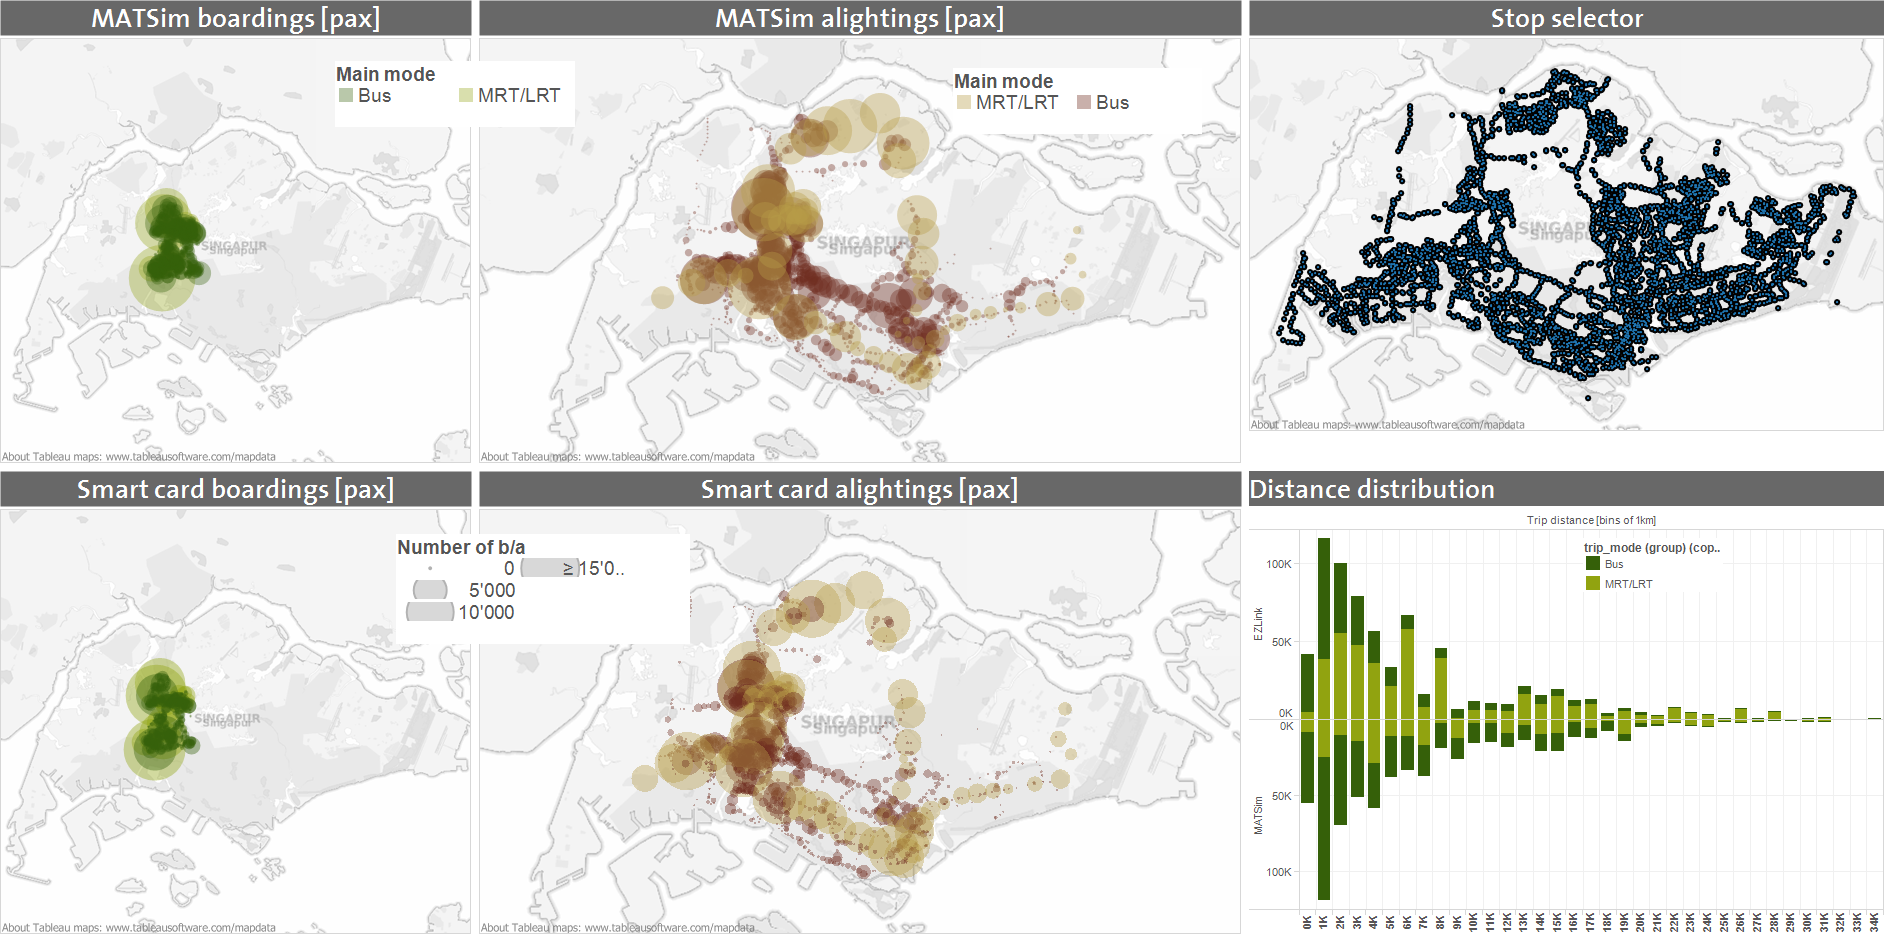
\includegraphics[width=0.25\textwidth, angle=0]{extending/figures/businessanalytics/tableau.png}}%
{}
% ------------

% ------------
\createfigure%
{General framework of the decision support system}%
{General framework of the decision support system}%
{\label{fig:analyticsFramework}}%
{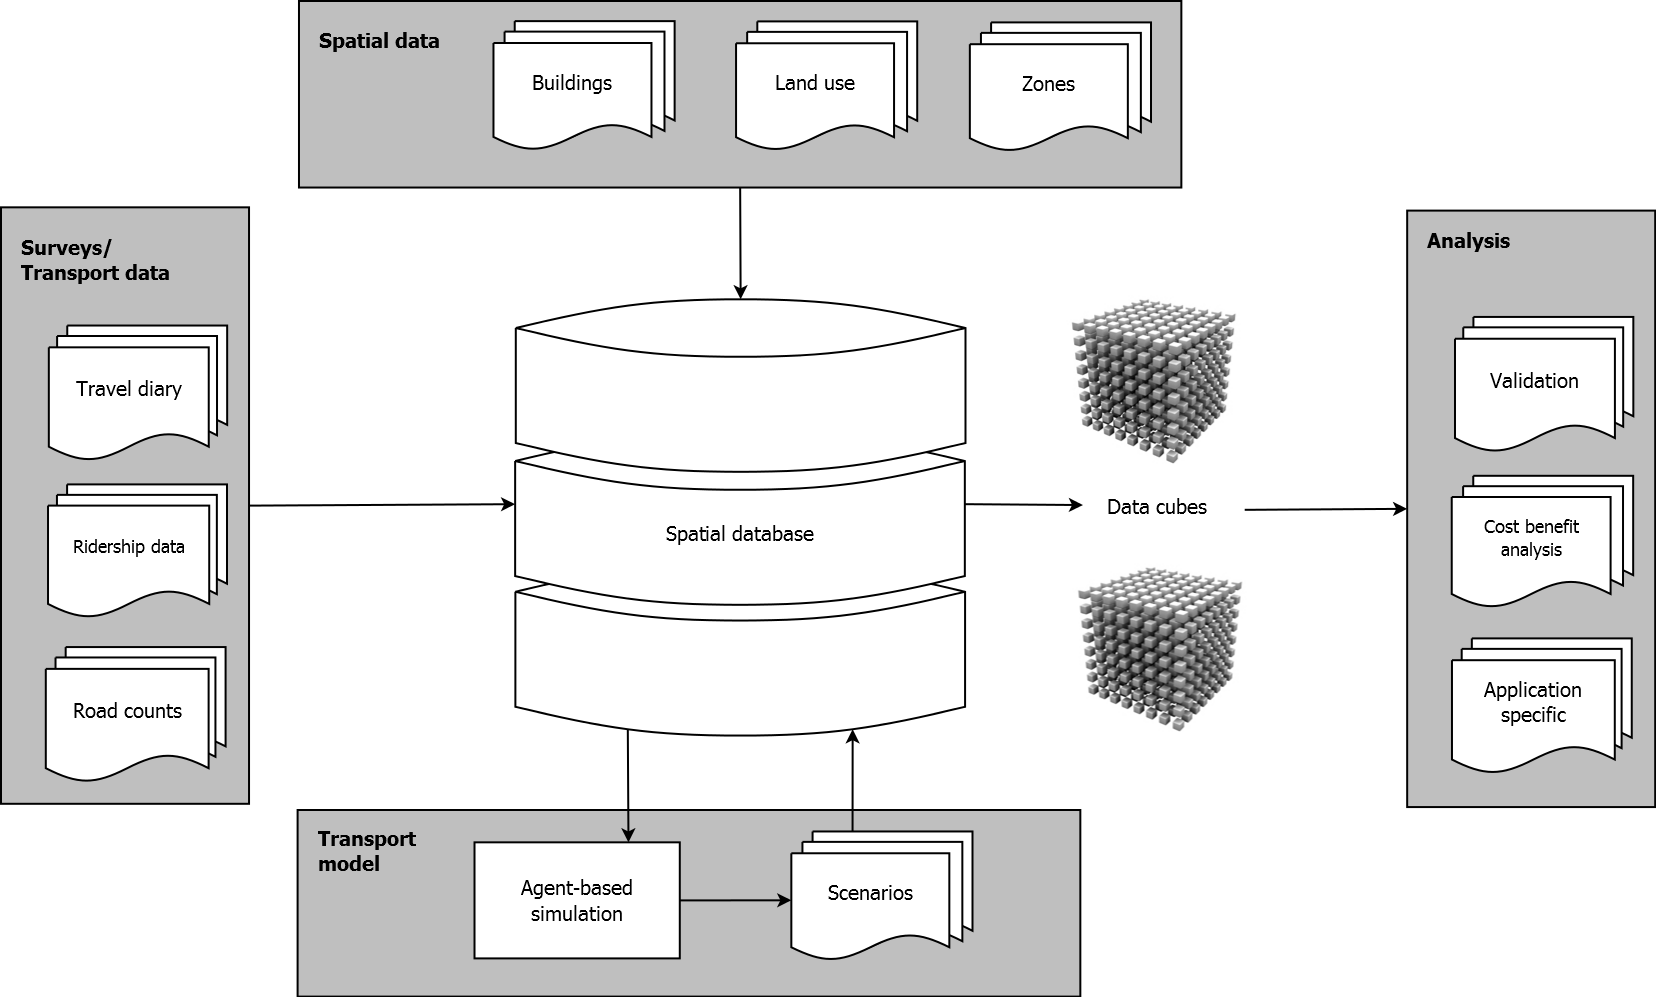
\includegraphics[width=0.65\textwidth, angle=0]{extending/figures/businessanalytics/general}}%
{}
% ------------

% ------------
\createfigure%
{Simplified entity relationship diagram showing shared keys across tables}%
{Simplified entity relationship diagram showing shared keys across tables}%
{\label{fig:analyticsERD}}%
{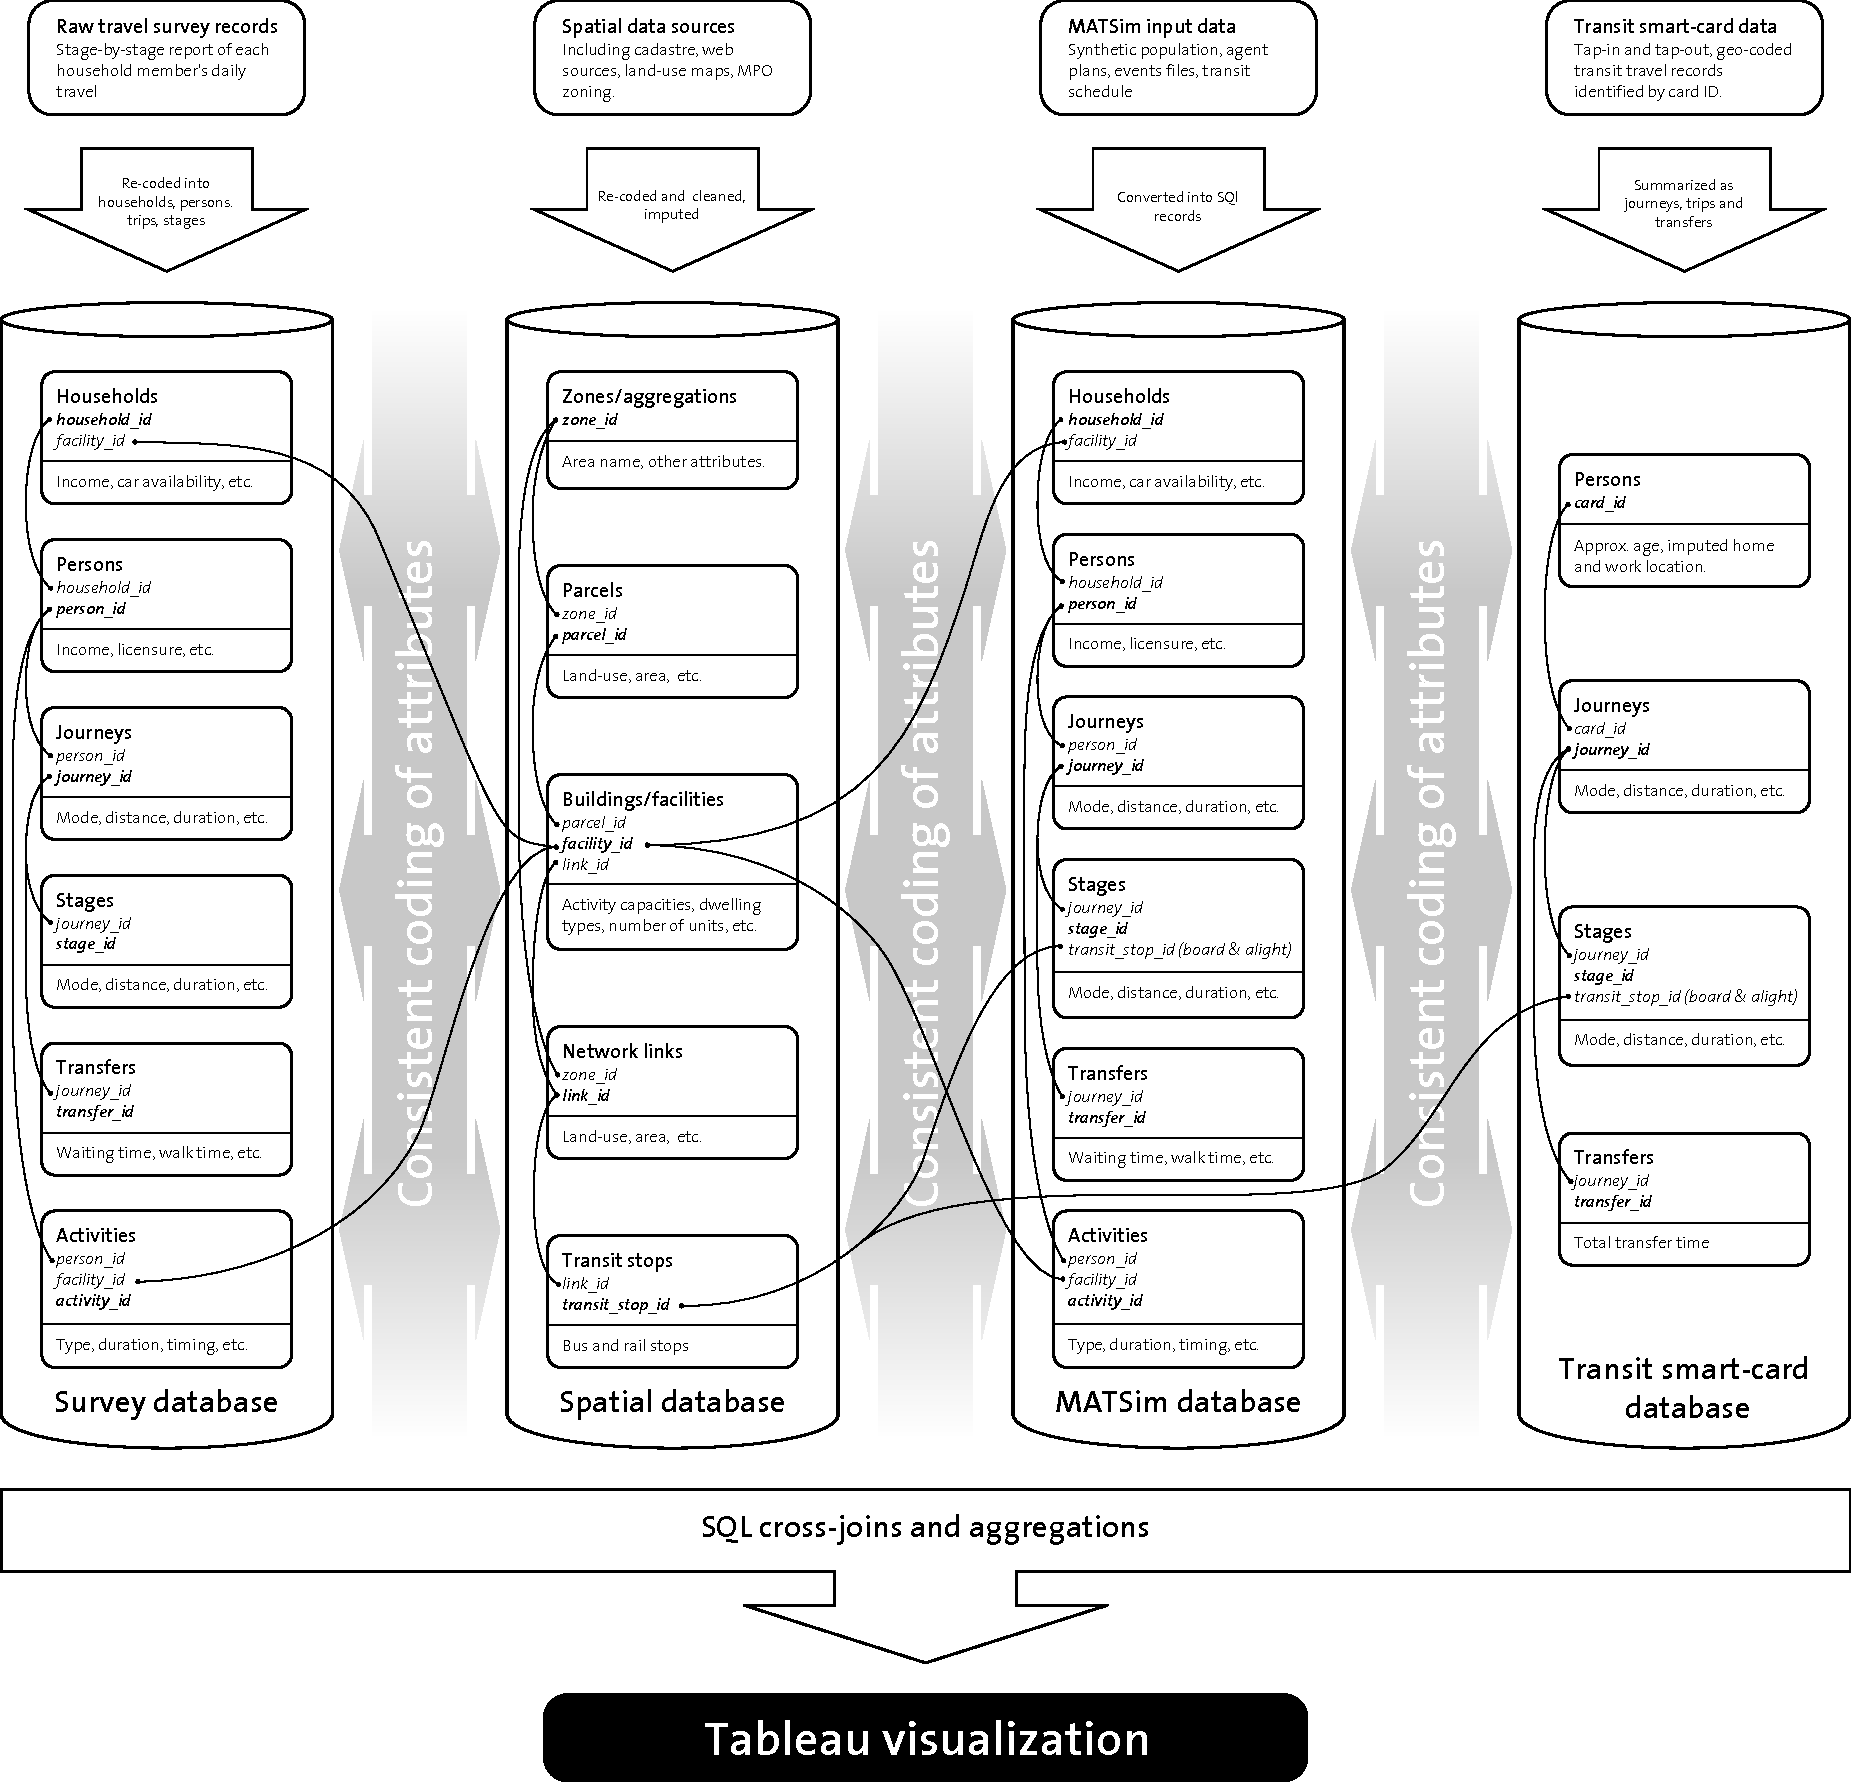
\includegraphics[width=0.65\textwidth, angle=0]{extending/figures/businessanalytics/schema}}%
{}
% ------------

% ------------
\createfigure%
{Table joined in analytics software}%
{A diagram showing how the tables from Figure \ref{fig:analyticsERD} are joined together for visualization in business analytics software, e.g. Tableau, as shown in Figure~\ref{fig:analyticsTableau}}%
{\label{fig:analyticsFramework}}%
{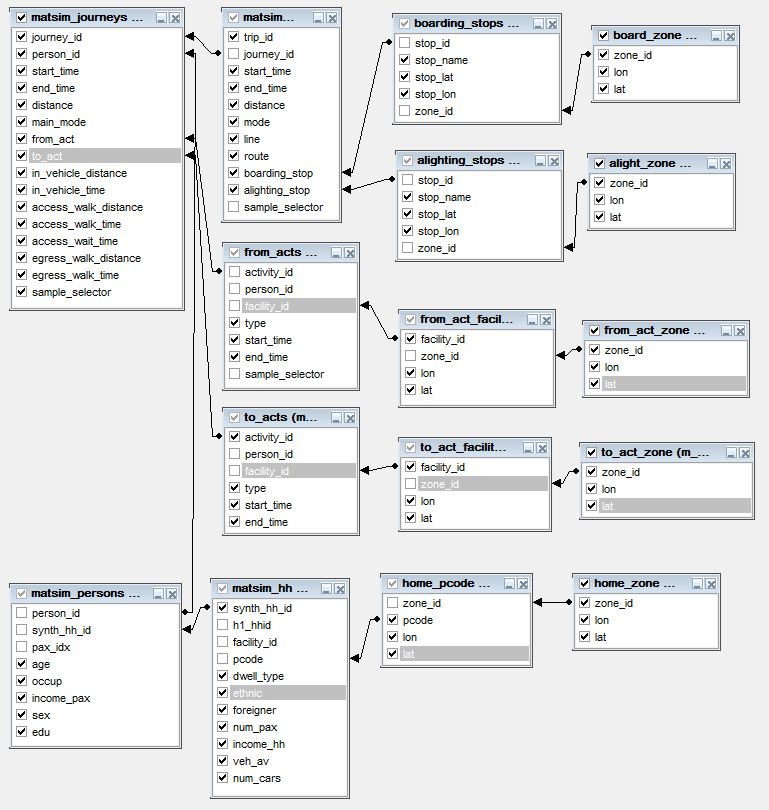
\includegraphics[width=0.65\textwidth, angle=0]{extending/figures/businessanalytics/join}}%
{}
% ------------



% ################################################################################################################
\section{Diaries from Events}
In the package \lstinline|playground.singapore.travelsummary| the reader may find a set of classes that will transform their MATSim simulation results into a set of travel diary tables, such as those discussed in the preceding section.

% ################################################################################################################




